\documentclass[12pt]{article}

\usepackage{url}
\usepackage{geometry}
\geometry{a4paper}
\usepackage{microtype}

\usepackage{graphicx}
\usepackage{amsmath}
\usepackage{algorithm}
\usepackage[noend]{algpseudocode}
\usepackage{float}
\usepackage{wrapfig}
\usepackage{listings}
\usepackage{multirow}
\usepackage{hyperref}

\usepackage{enumitem}

%para escribir en español
\usepackage[utf8x]{inputenc}
\usepackage[spanish]{babel}

\renewcommand{\contentsname}{Índice}
\renewcommand{\refname}{Referencias}
\renewcommand{\figurename}{Figura}

\usepackage[nottoc,numbib]{tocbibind}

\linespread{1.2}

\graphicspath{{./figures/}} % Specifies the directory where pictures are stored

\begin{document}

\begin{titlepage}

    \center

    \textsc{\LARGE Universidad de la República}\\[1.5cm]
    \textsc{\Large Facultad de Ingeniería}\\[1.0cm]
    \textsc{\large Recuperación de Información y Recomendaciones en la Web}\\[0.5cm]

    \rule{\linewidth}{0.5mm} \\[1cm]
    {\huge \bfseries Amazon Copilot}\\[0.5cm]
    \rule{\linewidth}{0.5mm} \\[1.5cm]

    \begin{minipage}{0.4\textwidth}
        \begin{flushleft} \large
            \emph{Autores:}\\
            Juan Pablo Conde\\
            Xavier Iribarnegaray\\
            Juan Pablo Sotelo\\
        \end{flushleft}
    \end{minipage}
    ~
    \begin{minipage}{0.4\textwidth}
        \begin{flushright} \large
            \emph{Profesores:} \\
            Libertad Tansini \\
        \end{flushright}
    \end{minipage}\\[2cm]

    {\large \today}\\[1.5cm]

    
\includegraphics[width=0.4\textwidth]{fing-logo}\\[1cm]

    \vfill

\end{titlepage}


\pagenumbering{arabic}

\tableofcontents

\newpage

\section{Introducción}
Amazon Copilot constituye un sistema diseñado para optimizar la búsqueda y selección de productos en plataformas de comercio electrónico. Basado en un conjunto de datos de productos de Amazon, el sistema implementará técnicas avanzadas de recuperación de información y procesamiento de lenguaje natural para proporcionar una experiencia de compra intuitiva y personalizada.

El proyecto integra tres funcionalidades principales: un sistema de búsqueda híbrido que combina técnicas semánticas y tradicionales para ofrecer resultados más relevantes; un asistente conversacional (Agente de Inteligencia Artificial) que proporciona una interfaz de búsqueda interactiva, refinando requerimientos mediante diálogo natural y utilizando como mecanismo subyacente el sistema de búsqueda híbrido implementado; y un sistema de recomendación que, basándose en los productos seleccionados en el carrito, emplea el mismo agente para identificar artículos similares o complementarios, mejorando así la experiencia de descubrimiento de productos.

\section{Funcionalidades del Sistema}

En esta sección se presentan las tres principales funcionalidades que se implementarán en Amazon Copilot.

\subsection{Búsqueda Híbrida de Productos}

Este componente combina técnicas de búsqueda semántica con métodos tradicionales de correspondencia textual para optimizar resultados. Incorpora representaciones vectoriales semánticas (embeddings) para capturar el significado contextual de las consultas, mantiene búsqueda por términos exactos para consultas específicas e implementa filtrado por categorías. El sistema ordena los resultados mediante un modelo que pondera tanto la relevancia semántica como la coincidencia sintáctica tradicional, logrando un equilibrio óptimo que aprovecha las fortalezas de ambos enfoques para mostrar los productos más pertinentes al usuario.

\subsection{Búsqueda Conversacional con Agente de IA}

El asistente conversacional proporciona una interfaz de búsqueda interactiva en lenguaje natural. Este agente mantiene el contexto durante la conversación, refina progresivamente los requerimientos del usuario mediante preguntas específicas, y utiliza la API de búsqueda híbrida como herramienta subyacente para ofrecer resultados personalizados. Resulta especialmente útil para usuarios sin conocimientos específicos sobre los productos que buscan.

\subsection{Sistema de Recomendación con Agente de IA}

Este sistema analiza los productos seleccionados en el carrito para sugerir artículos complementarios o alternativos. Opera automáticamente al visualizar el carrito, generando recomendaciones basadas en productos frecuentemente adquiridos conjuntamente y alternativas similares. Presenta explicaciones concisas sobre cada recomendación y adapta las sugerencias dinámicamente según el contenido del carrito y el historial de la conversación con el usuario.

\newpage

\section{Arquitectura del Sistema}

Esta sección describe los componentes principales del sistema, sus responsabilidades e interacciones, así como las tecnologías propuestas para su implementación.

\vspace{1cm}

\begin{figure}[H]
    \centering
    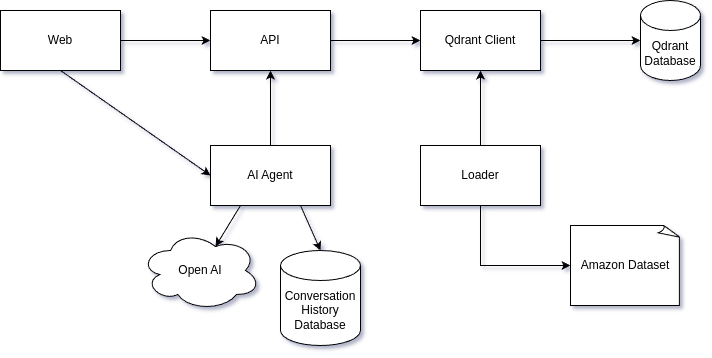
\includegraphics[width=0.8\textwidth]{architecture.png}
    \caption{Diagrama de alto nivel de la arquitectura del sistema.}
    \label{fig:system_architecture}
\end{figure}

\subsection{Web}

Este módulo define la interfaz gráfica y las interacciones del usuario con el sistema (UI/UX), constituyendo el frontend de la aplicación. A través de esta capa, los usuarios pueden acceder a todas las funcionalidades del sistema de manera intuitiva y eficiente.

\subsubsection{Diseño UX}

\begin{figure}[H]
    \centering
    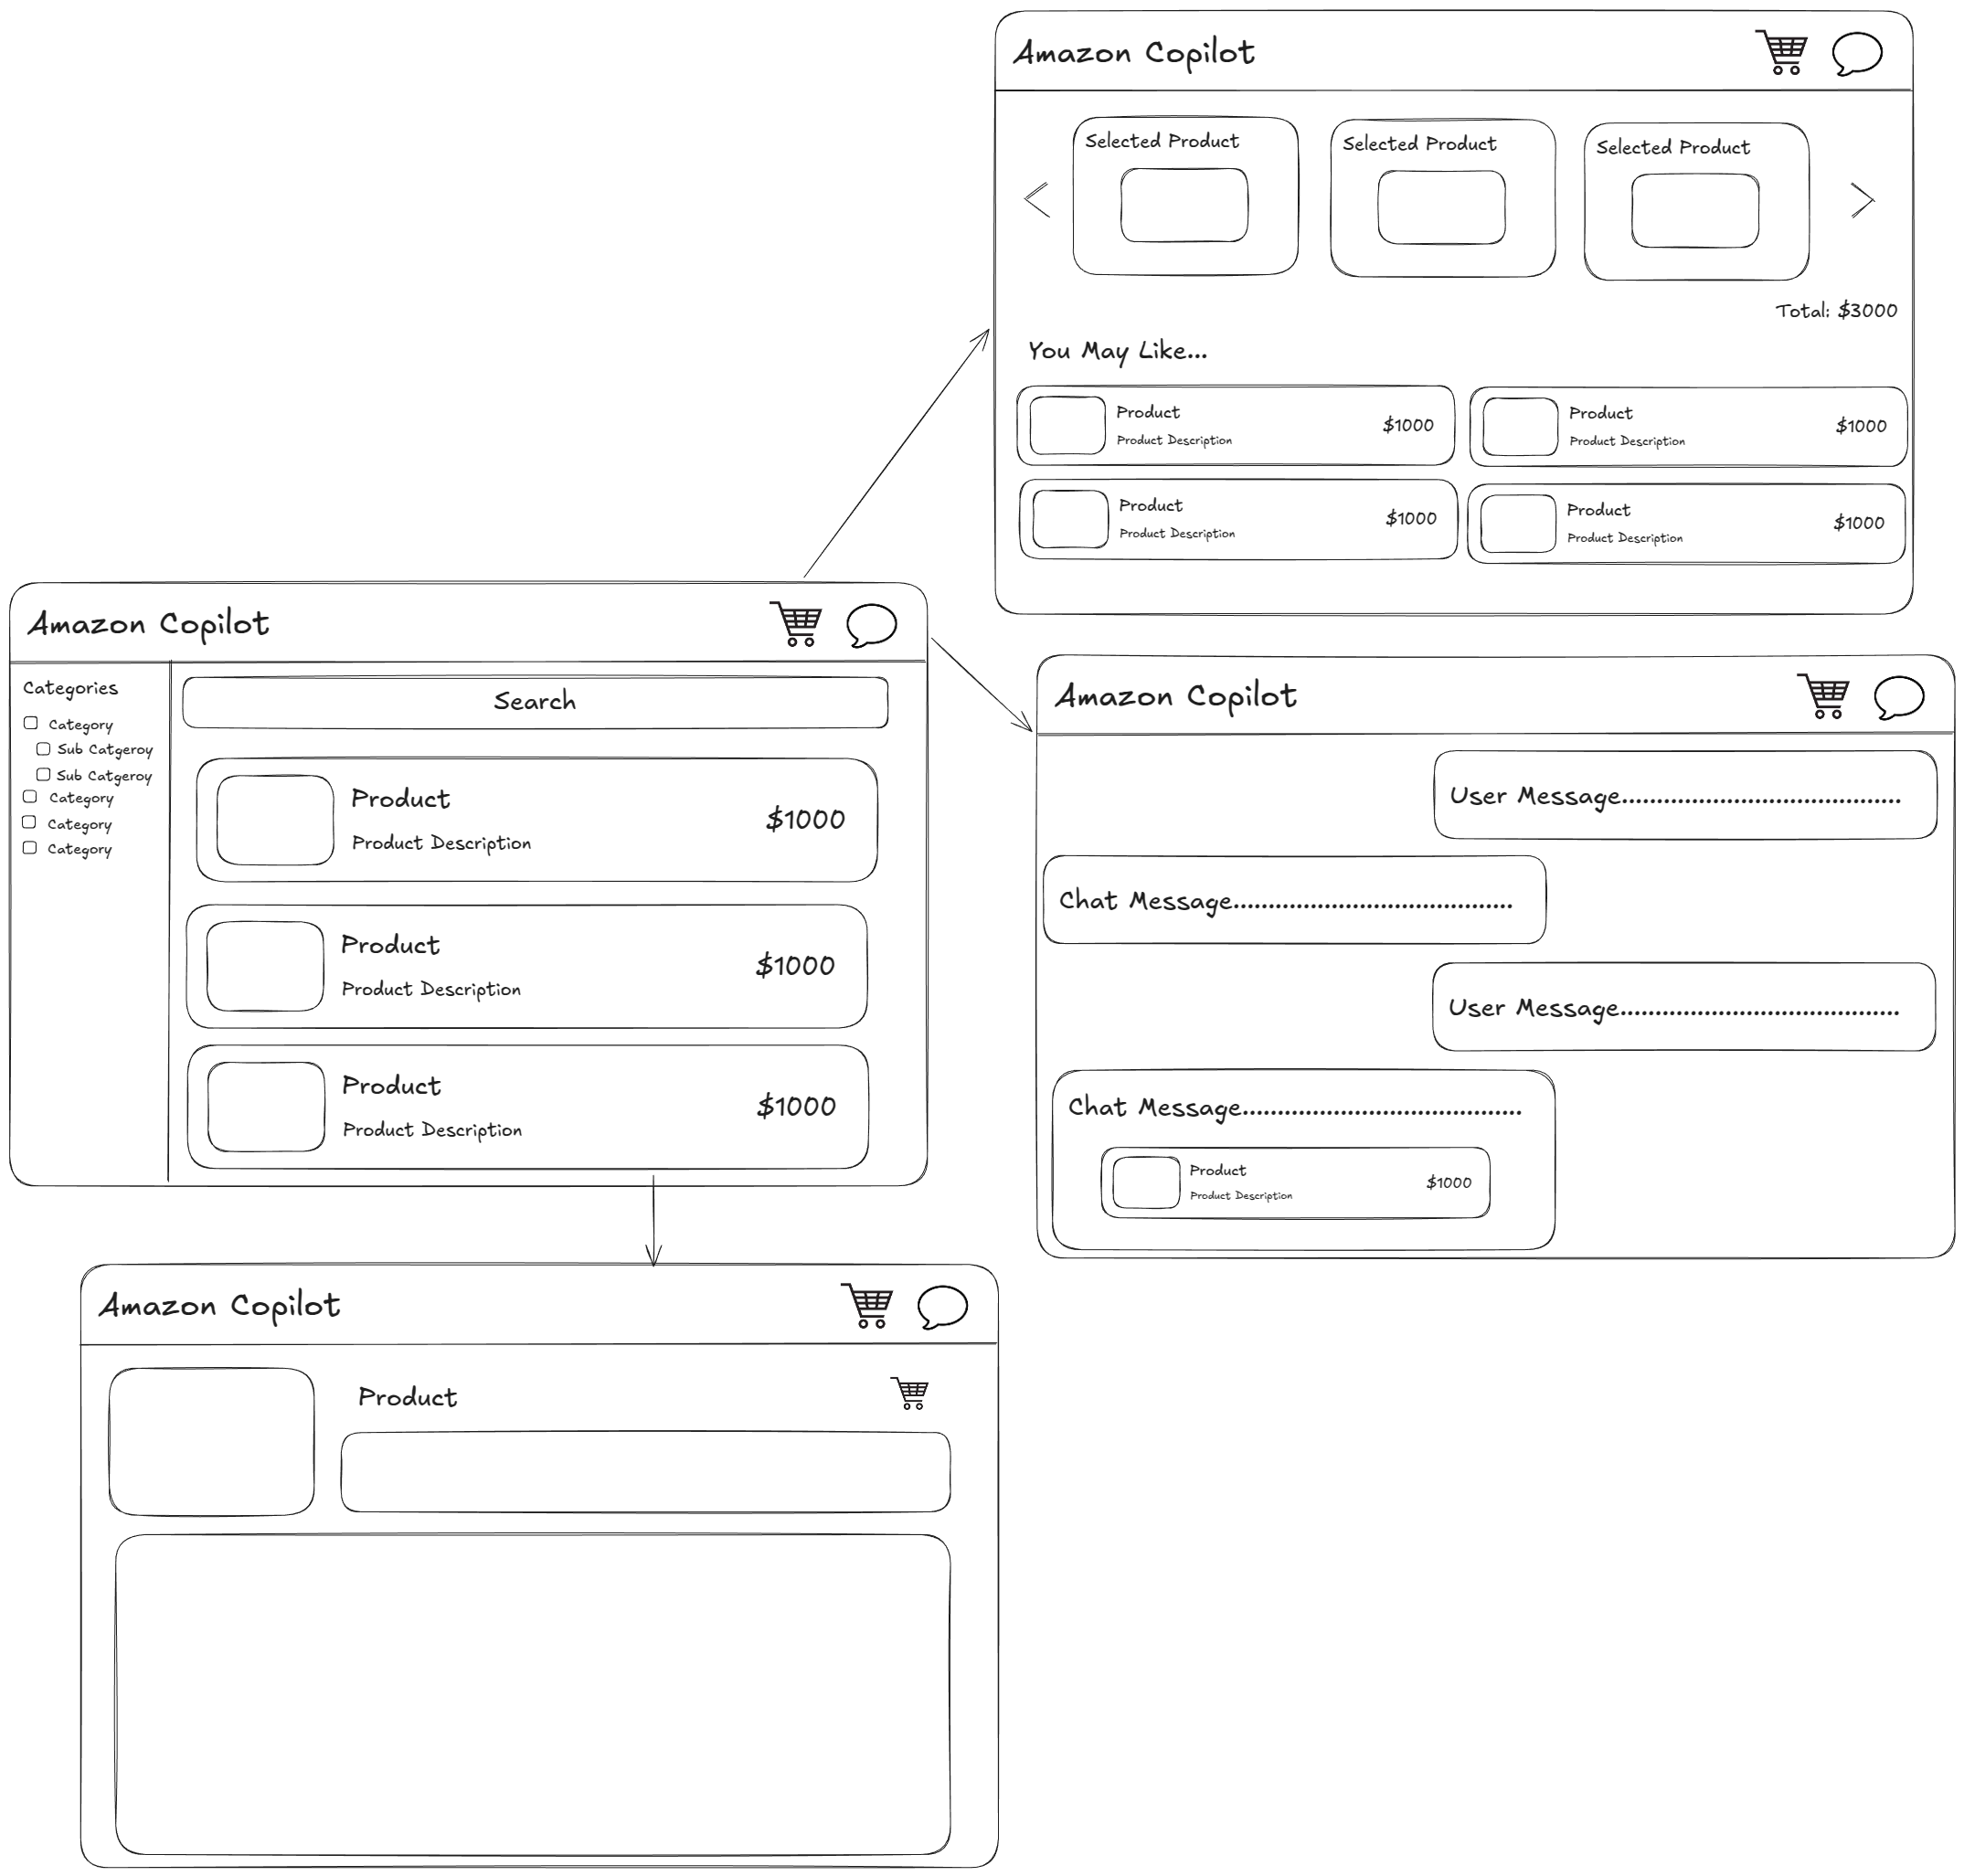
\includegraphics[width=0.8\textwidth]{ux.png}
    \caption{Diseño UX de la interfaz web.}
    \label{fig:ux_design}
\end{figure}

\noindent \textit{Nota: Este diagrama modela las interacciones del usuario con el sistema. El diseño final de la interfaz de usuario está pendiente de desarrollo.}

\vspace{0.75cm}

La interfaz permite al usuario: visualizar un listado inicial de productos con barra de búsqueda y filtros por categorías; realizar búsquedas que actualizan dinámicamente los resultados; acceder a detalles de productos específicos; gestionar un carrito de compras que muestra recomendaciones relacionadas; e interactuar con el asistente conversacional para búsquedas conversacionales, manteniendo el historial de la conversación.

\subsubsection{Implementación}

Dado que el objetivo principal del proyecto se centra en la funcionalidad de búsqueda y en el desarrollo del AI Agent, para el frontend adoptaremos la técnica de ``Vibe Coding'', utilizando herramientas como \href{https://www.cursor.com}{Cursor}~\cite{Cursor} y \href{https://replit.com}{Replit}~\cite{Replit}.

\begin{quote}
    ``There's a new kind of coding I call 'vibe coding', where you fully give in to the vibes, embrace exponentials, and forget that the code even exists. It's possible because the LLMs (e.g. Cursor Composer w Sonnet) are getting too good. [...] I'm building a project or webapp, but it's not really coding - I just see stuff, say stuff, run stuff, and copy paste stuff, and it mostly works.''
\end{quote}

\textit{Andrej Karpathy, \href{https://x.com/karpathy/status/1886192184808149383}{X}}~\cite{Karpathy}

\vspace{0.5cm}

Esta filosofía de desarrollo, asistida por modelos de lenguaje avanzados, nos permitirá iterar rápidamente sobre prototipos funcionales, concentrando nuestros esfuerzos técnicos en los componentes de búsqueda, recomendación e inteligencia artificial que constituyen el verdadero valor del proyecto.

\subsection{API}

Este componente constituye la capa de servicios que comunica el frontend con los distintos motores de búsqueda y recomendación. Incluye endpoints para listar productos (recibiendo parámetros de filtros y búsqueda) y para obtener información detallada de productos específicos.

\subsubsection{Implementación}

La API será implementada utilizando \href{https://fastapi.tiangolo.com/}{FastAPI}~\cite{FastAPI}, un framework moderno de Python que permite un desarrollo eficiente y robusto. FastAPI ofrece validación automática de datos mediante \href{https://docs.pydantic.dev/latest/}{Pydantic}~\cite{Pydantic}, tipado estático que reduce errores en tiempo de desarrollo, y generación automática de documentación con OpenAPI y Swagger UI. Esta documentación servirá como recurso valioso para la fase de desarrollo del frontend.

\subsection{Agente de IA}

Este componente implementa la funcionalidad conversacional y de recomendación del sistema utilizando \href{https://www.langchain.com/langgraph}{LangGraph}~\cite{LangGraph} y los modelos generativos de \href{https://openai.com/}{OpenAI}~\cite{OpenAI}. Utiliza la API de búsqueda híbrida como herramienta para acceder a los productos, permitiendo una arquitectura donde el diálogo con el usuario y la obtención de información están claramente separados.

Para mantener el contexto de las interacciones, el sistema se integra con una base de datos que almacena el historial de conversaciones, permitiendo referencias a consultas anteriores y facilitando la personalización progresiva de las respuestas.

\subsection{Qdrant}

Este módulo constituye el núcleo del sistema de búsqueda vectorial. Se compone de:

\begin{itemize}
    \item \textbf{Base de datos vectorial}: Almacena productos y sus representaciones vectoriales (embeddings densos y esparsos), permitiendo búsquedas por similitud y coincidencia exacta.

    \item \textbf{Cliente de acceso}: Componente que gestiona las operaciones de indexación y consulta a la base de datos. Implementa búsqueda híbrida siguiendo las prácticas recomendadas por \href{https://qdrant.tech/documentation/search-precision/reranking-hybrid-search/}{Qdrant}~\cite{Qdrant}, combinando embeddings densos (para capturar significado semántico) y esparsos (para coincidencias textuales precisas), permitiendo así obtener resultados relevantes tanto para consultas conceptuales como específicas.
\end{itemize}

La separación de este módulo facilita adaptaciones futuras, permitiendo reemplazar modelos de embeddings o migrar a soluciones alternativas sin impactar al resto del sistema.

\subsection{Dataset}

Para la información de productos, se utilizará el conjunto de datos de Amazon disponible en \href{https://www.kaggle.com/datasets/lokeshparab/amazon-products-dataset/data?select=Amazon-Products.csv}{Kaggle}~\cite{Amazon}. Este conjunto de datos ofrece una amplia variedad de atributos por producto, incluyendo:

\begin{itemize}
    \item Título y descripción detallada
    \item Categorías y subcategorías
    \item Precio y disponibilidad
    \item Valoraciones y número de reseñas
    \item Imágenes de productos
    \item Especificaciones técnicas
\end{itemize}

La riqueza de estos atributos permitirá implementar las modalidades de búsqueda previamente mencionadas.

Para la carga inicial del conjunto de datos, se desarrollará un módulo de carga consistente en scripts de Python que procesarán el archivo CSV, transformarán los datos en el formato requerido y utilizarán la funcionalidad de almacenamiento del cliente de Qdrant para indexar cada producto.

\newpage

\begin{thebibliography}{2}
    \raggedright

    \bibitem{Cursor}Cursor. (2024). \textit{Cursor: The AI-first code editor}. \url{https://www.cursor.com}

    \bibitem{Replit}Replit. (2024). \textit{Replit: The collaborative browser based IDE}. \url{https://replit.com}

    \bibitem{Karpathy}Karpathy, A. (2023, 11 noviembre). \textit{Tweet sobre "vibe coding"}. X. \url{https://x.com/karpathy/status/1886192184808149383}

    \bibitem{FastAPI}FastAPI. (2024). \textit{FastAPI: Framework web de alto rendimiento para APIs con Python}. \url{https://fastapi.tiangolo.com}

    \bibitem{Pydantic}Pydantic. (2024). \textit{Pydantic: Validación de datos para Python}. \url{https://docs.pydantic.dev/latest}

    \bibitem{LangGraph}LangGraph. (2024). \textit{LangGraph: Orchestration framework for building stateful, multi-actor applications with LLMs}. \url{https://www.langchain.com/langgraph}

    \bibitem{OpenAI}OpenAI. (2024). \textit{OpenAI: Creating safe AI that benefits humanity}. \url{https://openai.com}

    \bibitem{Qdrant}Qdrant. (2024). \textit{Qdrant: Vector Database}. \url{https://qdrant.tech/documentation/search-precision/reranking-hybrid-search}

    \bibitem{Amazon}Parab, L. (2023). \textit{Amazon Products Dataset}. Kaggle. \url{https://www.kaggle.com/datasets/lokeshparab/amazon-products-dataset/data?select=Amazon-Products.csv}

\end{thebibliography}

\end{document}
